\documentclass[a4paper]{article}
\usepackage{ctex}
\usepackage{enumitem}
\usepackage{multirow}
\usepackage{fancyhdr}
\usepackage{amsmath}
\usepackage{parskip}
\usepackage{float}
\usepackage{hyperref}
\usepackage{listings}
\usepackage{xcolor}

\setlength{\parskip}{6pt}

\pagestyle{headings}

% GitHub styles
\definecolor{keyword}{HTML}{CF222E}
\definecolor{comment}{HTML}{6E7781}
\definecolor{string}{HTML}{0A3069}

\lstset{
    commentstyle=\color{comment},
    keywordstyle=\color{keyword},
    stringstyle=\color{string},
    basicstyle=\ttfamily\small,
    breakatwhitespace=false,
    breaklines=true,
    captionpos=b,
    keepspaces=true,
    showspaces=false,
    showstringspaces=false,
    showtabs=false,
}

\begin{document}
\title{四子棋实验}
\author{梁业升 2019010547(计03)}

\maketitle

评测结果:\hyperlink{https://www.saiblo.net/batch/23993}{https://www.saiblo.net/batch/23993}。

\begin{tabular}{c c c c}
    胜 & 平 & 负 & 胜率 \\
    \hline
    87 & 0 & 13 & 87\%

\end{tabular}

\section{算法概述}\label{sec:algorithm}

使用蒙特卡洛树搜索算法。

\begin{figure}[H]
\centering
    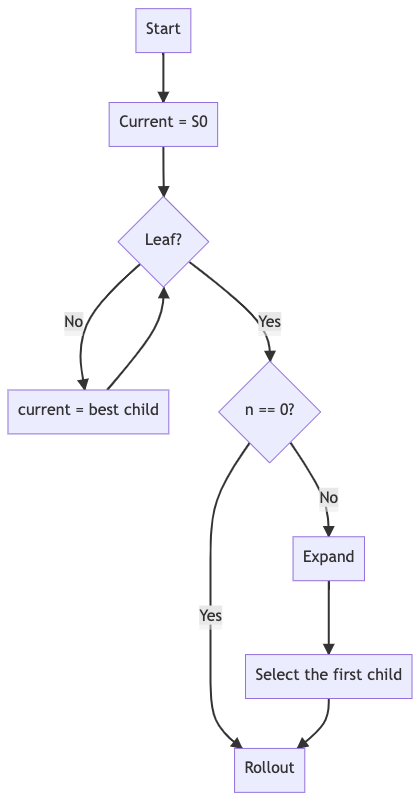
\includegraphics[width=0.4\textwidth]{assets/mcts.png}
    \caption{蒙特卡洛树搜索算法}
\end{figure}

子节点的选择使用信心上限算法:

$$I_j=\overline{X}_j+c\sqrt{\frac{2\log N}{N_j}}$$

其中:

\begin{itemize}
    \item $\overline{X}_j$ 为第 $j$ 个子节点的平均收益(获胜为 1,打平为 0,失败为 -1)
    \item $N$ 为父节点访问的总次数
    \item $N_j$ 为第 $j$ 个子节点被访问的次数
\end{itemize}

在本实验中,$c$ 选择 $0.55$。

\section{实现方法}\label{sec:method}

在基本的信心上限树算法的基础上,采取了一些优化方案,较大地改善了 AI 的性能。

\subsection{人工干预}

为避免搜索深度不够而导致对某些紧急情况过于乐观或对某些有利局面过于悲观,在使用信心上限树进行模拟前后进行了两次人工干预。
因为只进行一次,所以既不会对模拟次数产生影响,同时又能防止 AI 下臭棋或错失好局。

在进行模拟前:

\begin{enumerate}
    \item 分析本方是否有必胜的下棋位置,若有,立即返回此位置,即获得胜利。
    \item 分析当前对手是否有在某个位置下棋而获得胜利的可能,若有,立刻返回此位置以“救火”。
    \item 分析本方是否有创造两个必胜下棋点的可能,若有,再次判断此步棋是否有可能为对手创造必胜局面,
          \begin{itemize}
              \item 若有,则放弃此步棋,进行模拟。
              \item 若无,则立即返回此位置,下一步棋必有必胜局面。
          \end{itemize}
\end{enumerate}

在进行模拟后,对根节点的各个子节点:

\begin{enumerate}
    \item 分析对手在本方下此位置后是否有在某个位置下棋而获得胜利的可能,若有,放弃此位置,而不管其分数高低。
    \item 分析对手在本方下此位置后是否有创造两个必胜下棋点的可能,若有,尽量放弃此位置。
\end{enumerate}

然后,返回剩余节点中分数最高的节点。如果没有剩余节点,则返回必输节点外分数最高的位置;如果只有必输节点,则返回第一个。

\subsection{Rollback 剪枝}

在进行 Rollback 的过程中,每次随机选择下棋位置前,先判断下在此位置后是否能够导致游戏结束,若是,则直接返回,不再随机。这样的好处是在胜负已定的时候能够避免大量无意义的随机,提高搜索的深度。

\subsection{加速胜负判断}

使用位棋盘(Bitboard)加速胜负判断。一个 64 位的位棋盘的排布如下:

\begin{lstlisting}
  6 13 20 27 34 41 48   55 62     additional row
+---------------------+ 
| 5 12 19 26 33 40 47 | 54 61     top row
| 4 11 18 25 32 39 46 | 53 60
| 3 10 17 24 31 38 45 | 52 59
| 2  9 16 23 30 37 44 | 51 58
| 1  8 15 22 29 36 43 | 50 57
| 0  7 14 21 28 35 42 | 49 56 63  bottom row
+---------------------+    
\end{lstlisting}

实现中使用 \texttt{g++} 内置的 \texttt{\_\_int128\_t} 实现 128 位棋盘。判断当前某方是否胜利时,只需进行 15 次位运算、2 次加法运算和 3 次乘法运算:

\begin{lstlisting}[language=C++]
inline bool hasWon(Side side) {
    __int128_t diag1 = board & (board >> height);
    __int128_t hori = board & (board >> (height + 1));
    __int128_t diag2 = board & (board >> (height + 2));
    __int128_t vert = board & (board >> 1);
    return ((diag1 & (diag1 >> (2 * height))) |
            (hori & (hori >> (2 * (height + 1)))) |
            (diag2 & (diag2 >> (2 * (height + 2)))) |
            (vert & (vert >> 2)));
}
\end{lstlisting}

由于棋盘规模最大为 $12\times 12=144$,大于 128,因此对于不能使用位棋盘的情形,我们使用原始的数组表示和计算。

经测试,使用位棋盘大约能给总体带来将近 1 倍的性能提升(局面判断本身快几个数量级)。

\subsection{一些实现细节}

\subsubsection{节点池}

预先分配一个节点池用于新建节点,无需动态分配内存。每次模拟可重复利用。

\subsubsection{问题排查}

使用条件编译的方法,针对本地 DEBUG 环境进行输出或检查:

\begin{lstlisting}[language=C++]
#ifdef DEBUG
#define print(fmt, ...) printf(fmt, ##__VA_ARGS__)
#define myAssert(e) assert(e)
#define debug(s) s
#else
#define print(fmt, ...) ;
#define myAssert(e) ;
#define debug(s) ;
#endif
\end{lstlisting}

这样可以在不影响在线评测的情况下,很方便地查看输出、排查问题。比如,对某些条件进行 \texttt{assert}:

\begin{lstlisting}[language=C++]
myAssert(lastChoice >= 0);
myAssert(columnAvailable(lastChoice));
\end{lstlisting}

对死循环进行检测:


\begin{lstlisting}[language=C++]
debug(int loopCount = 0);
while (current != root) {
    ...
    debug(loopCount++);
    debug(myAssert(loopCount < 10000));
}
\end{lstlisting}

另外,还实现了对模拟的各个过程用时的记录:

\begin{lstlisting}[language=C++]
debug(start = clock());
backup(current, result);
debug(backupTime += clock() - start);

// Restore board and top
debug(start = clock());
restoreBoardAndTop();
debug(restoreTime += clock() - start);
\end{lstlisting}

每次模拟结束后,可以观察各个部分的用时:

\begin{lstlisting}[language=C++]
Recorded time: 86.51%
Traversal time: 16.80%
Rollout time: 59.33%
Expand time: 1.61%
Restore time: 5.45%
Backup time: 3.31%
\end{lstlisting}

这有助于优化性能瓶颈,例如曾经借助此信息解决了恢复棋盘用时过长而导致搜索性能下降等问题。

\end{document}
